\documentclass[letterpaper,11pt]{article}
\usepackage[textwidth=6.5in,textheight=8.5in]{geometry}
\usepackage{graphicx}
\usepackage{fancyhdr}
\usepackage{array}
\usepackage{amsmath}
%document font (Times)
\usepackage{tgtermes}
\usepackage[T1]{fontenc}
%\usepackage{mathptmx}
\usepackage{enumitem}

%\hoffset=-0.74in
%\voffset= -0.8in
%\textwidth=6.5in
%\textheight=8.5in
%\marginparwidth=0pt

%\fancyhead{}
%\fancyfoot{}
%\pagenumbering{Roman}
\lhead{\includegraphics[width=0.25\textwidth]{../figures/C-3logo.png}}
\chead{}
\rhead{}
%\cfoot{Mailing Address: \\Tel: 1(703)}

\pagestyle{fancy}

%\title{\bf{Self-Organizing Interference Alignment (SOIA)\\for Tactical Mobile Edge Networks}}


\begin{document}

%\thispagestyle{fancy}

%\maketitle

\begin{center}
~\\
~\\
~\\
{\Large{\huge\bf{Self-Organizing Interference Alignment (SOIA) for Tactical Mobile Ad Hoc Communications Network}}}\\
~\\
\vspace{0.1in}
Zhongren Cao\\
zcao@c3commsystems.com
\end{center}

\vspace{0.1in}

\begin{abstract}
Theoretical studies have shown the interference alignment has the potential to significantly improve the capacity of a wireless network. However, realizing interference alignment in practical networks requires costly coordination overhead, which may cancel out the gains obtained from interference alignment. In addition, it is a challenging task to group multiple transceiver pairs for interference alignment in a mobile ad hoc network where there is no centralized control.This proposal introduces self-organizing interference alignment (SOIA), a distributed approach for constructing clusters of transceiver pairs to perform interference alignment in a tactical mobile ad hoc communication network (TMACN). SOIA significantly reduces the coordination overhead by computing solutions locally at each individual receiver without requiring the channels of other receivers. SOIA leverages existing TMACN medium access control (MAC) scheme, thus it enables the seamless coexistence of  SOIA and non-SOIA radio nodes in the same network. The resulting SOIA product is expected to have low cost and supports a phased roll-out for speedy deployment without causing disruptions to existing equipment. In the proposed phase I and phase I option effort, we will develop the SOIA approach, comparatively evaluate its performance in simulation, and design a detailed Phase II prototyping and demonstration plan.
\end{abstract}

\newpage

\section{IDENTIFICATION \& SIGNIFICANCE OF THE OPPORTUNITY}

\subsection{Problem Identification}
Epitomized by recent military operations, modern warfare is conducted by small units at tactical edges. The 2012 new strategic guidance for Department of Defense articulates that one of the primary missions of the U.S. Armed forces is to project power despite anti-access/area denial (A2AD) challenges~\cite{DoD:strategy2012}, including implementing the Joint Operational Access Concept~\cite{DoD:JOAC}, which suggests ``smaller units and platforms that are rapidly deployable yet lethal." For warfighters in small units at tactical edges, efficiently sharing real-time situational awareness information is critical to their mission success. To this end, the tactical Mobile Ad hoc Communications Network (TMACN) is important because it will provide the backbone for exchange and sharing of information from sensors, manned and unmanned vehicles and systems, and dismounted soldiers. Improving the network capacity for TMACN has a direct impact on warfighter's mission success . 

%Some of the unique features that distinguish TMACNs from traditional wireless networks are their mobility; they must be self contained and have the ability to move to support forces as engagements change, their adaptability; they must be able to reconfigure themselves in real-time as new nodes are added and others are lost, and their size; they may be on the order of hundreds or even thousands of nodes. The uniqueness associated with TMACNs gives rise to several complexities that limits a satisfactory solution for performance prediction; theories required to predict their performance have yet to be developed, and adequate hardware to test them is still years away. The focus of this effort is to develop a performance prediction solution for TMACNs based on simulation.

Wireless networks are interference limited due to the fact that multiple users need to share the transmission resources. Traditionally, time and frequency resources in wireless networks are divided into orthogonal units and assigned to different users, such as TDMA, FDMA and OFDMA. Each resource unit can only be used by a single transmission in order to avoid interference among multiple simultaneous transmissions. For large networks, resource reuse is widely adopted in both commercial and military systems to increase the network capacity. The same frequency/time resource unit is shared by multiple transceiver pairs that are far apart geographically such that mutual interference is not significant due to path loss. 

In addition to the frequency and the time signaling dimensions, multiple antenna arrays and MIMO systems enable the vector space as a third signaling dimension, i.e. the spatial dimension. The spatial dimension can be shared among multiple transmissions or multiple data streams of the same transceiver pair. The same time and frequency resource unit can be shared among multiple transmissions as long as they can be separated in the spatial dimension. In the ideal case, each transmission occupies a subspace that is orthogonal to the subspaces of all other parallel transmissions. In reality, due to correlations among antennas, the channel matrix may be rank-deficient thus limits the number of simultaneous transmissions that can be supported. To some extend, spread spectrum technology can also be viewed as using vector-based signaling to support multiuser communications. 

All aforementioned approaches are built upon the basic doctrine that, in order to avoid interference, closely located transceiver pairs in a wireless network must use orthogonal transmission resource units for simultaneous transmissions. Each resource unit can only be used by a single transmission. Therefore, the number of simultaneous transmissions are upper bounded by the number of orthogonal resource units available to use. Given the limited bandwidth each radio can access and the limited number of antennas each radio is equipped per size, weight and power (SWaP) requirements, the capacity of tactical mobile networks is thus constrained during operational deployment. 

In order to further enhance the capacity of tactical networks, we need to develop fundamentally new technology that can be deployed in realistic mission operations. 

\subsection{Interference Alignment -- The Opportunity for More Wireless Network Capacity}

Interference alignment (IA) is an emerging approach, which breaks away from the above fundamental doctrine, i.e., the number of simultaneous transmissions among closely located radio transceivers is limited by the number of orthogonal transmission resource units.  

 In interference alignment, the signaling of multiple closely located transceiver pairs are jointly designed, such that at each individual receiver all interference aligned into a subspace that is orthogonal to the desired signal. The number of interferences is more than the rank of the aligned subspace. This is explained graphically in Fig.*. ... Using interference alignment, from the network point of view, the number of simultaneous transmissions within the interference range can be more than the number of available orthogonal resource units. Thus, the overall network throughput is increased.

At least in theory, shows it can significantly improve the network capacity. The theoretic concept of interference has been extensively explained in many academia publications. The theoretic framework for IA has several idealistic assumptions that need to be addressed before apply IA in practical systems. First, since IA jointly design the transmission signals for multiple transmitters, the channel state information (CSI) is central to calculating IA beamforming vectors. As a result, IA incurs significant overhead for CSI estimations and feedback. In mobile fast-fading environment, the overhead of CSI acquisition can limit or cancel out the gains of IA. 

\subsection{Practical Challenges and Requirements}

Theoretical investigation shows that a $K$-pair interference channel with IA can achieve its total DOF, which is $K/2$ [\#].  In practice, several challenges have to be addressed before materializing the capacity gain promised by IA in an operational TMACN.

{\textbf{\textit{Clustering transceiver pairs}}} --- IA requires coordination among multiple transceiver pairs to design the signals and setup the joint transmissions in the physical layer. So the first step in applying IA is to cluster transceiver pairs instead of individual nodes, as in the traditional mobile ad hoc network (MANET) clustering problem  [\#]. Even given the same group of radios, if the pairing of transceivers changes, the IA signaling of this group has to be re-designed. Most research papers discussing IA assume that the $K$ pairs are given {\it{a prior}}. This assumption is reasonable for a cellular system, where a centralized control plane manages multiple base stations and also has the full knowledge of all traffic. The knowledge of current traffic needs is necessary to determine the participating transceiver pairs within a cluster. TMACN, on the contrary, doesn't have a centralized control plane. Each radio in TMACN knows only its own traffic needs. There is no entity in a TMACN which has global knowledge of all traffic needs. In short, distributed pairing of radios with active traffic need is the first challenge to be addressed.

{\textbf{\textit{Handling heterogeneous radios}}} ---  Tactical networks are inherently heterogeneous. Dismounted soldier radios and vehicle mounted radio transceivers have different SWaP requirements. Hence, different radios are equipped with various numbers of antennas. For example, the AN/PRC-154 Rifleman Radio that is being fielded now to combat troops is a single transceiver radio. The AN/PRC-155 Manpack radio has two radio channels. More antennas may be available on vehicular-mounted radios, for example AN/PRC-117G. Given the dynamic nature of battlefield communications, the IA solution computing must take into account the fact that, within an IA cluster, some radios have reduced signal dimensionality than the others. This indicates that each radio must share its antenna configuration with neighboring nodes to facilitate transceiver pair clustering and IA solution generation. 

{\textbf{\textit{Limiting coordination overhead}}} --- To compute IA solutions, classical IA algorithms requires not only the channel state information (CSI) of all participating transceiver pairs, but also the CSI of all interfering pairs. For a $K$-pair IA scheme, $K^2$ sets of CSI information are required for computing. To control the growth of coordination overhead, smaller clusters are preferable. Since IA engine must recalculate the IA precoder beamforms when the channel changes, coordination overhead also grows in high-mobility fast-fading environment, which is typical in tactical deployment. As a result, TMACN requires IA schemes that can significantly reduce the need for CSI acquisition feedback. Protocol level coordinations, such as determining the beginning and ending of the transmission, selecting time and frequency synchronization reference point, achieving synchronization, also incur overhead. An ideal solution for practical TMACN systems would achieve protocol level coordination with minimum cost.

In addition to above challenges, inserting new technology into military systems has to be an evolutional process, such that we can not only maximize the value of existing technology and capital investment, but also speed up the deployment of new technology. Applying IA into TMACN is no exception. We need to leverage existing TMACN operations when designing the approach to cluster IA transceivers pairs, and develop the algorithm for computing IA solutions. At times when IA is unfeasible or cannot offer expected capacity gains, radios must be able to continue operate in the conventional mode.

%In particular, tactical mobile ad hoc network (TMACN) poses several challenges to apply IA. 
%Several challenges have to be addressed in order to reap the benefits of IA in operational tactical mobile ad hoc network. 
%Second, unlikely commercial systems, TMACN usually doesn't have a centralized control plane. Therefore, IA relies on distributed coordination among peer nodes. 
%Third,  technology evolution instead of revolution is better for TMACN.
%Therefore, a distributed 
%First, tactical network is inherently heterogeneous.  size weight and power (SWaP) requirements 
% Situational awareness at tactical edge requires  higher data throughput
% Interference alignment overview and its potential application to improve the throughput of tactical edge network
% General challenges of applying interference alignment 
% Challenges posed by the tactical edge networks
%  1. Hybrid nodes (vehicle node vs. dismounted nodes) from one antenna to multiple antennas
%  2. Hierarchical network architecture
% It requires several steps to incorporate IA into the TMACN operations. The first step is to identify IA opportunities. 

\section{PHASE I TECHICAL OBJECTIVES}

% A self-organizing interference alignment scheme supporting distributed clustering
% Built on the existing medium access control schemes widely adopted in TMACN.  

The overall PHASE I technical objective is to investigate, design and evaluate an interference alignment scheme, which not only can improve the capacity of TMACN, but also is practical for prototyping, demonstration and transition. Specifically, this scheme should be able to dynamically form IA transceiver clusters without a central control plane,  operate flexibly with heterogeneous radio nodes, and significantly reduce coordination feedbacks. 

%The objectives of this proposal to develop a practical interference alignment scheme that is applicable to transmission scheme 

%In we propose to design a software suite, which enables distributed interference alignment cooperations among tactical edge mobile nodes.  Since most existing military waveforms operate in slotted or TDMA mode, THE SYSTEM assumes a operational slotted network without IA as the baseline. In order to be backward compatible with existing tactical protocols,  where initial slot assignment is assumed to be performed by methods used in existing TMACN, such as SRW. Thus, each node possesses a series of time slots. The system level gain from IA comes from enabling other transceiver pairs to share time slots assigned to node ??. 

\subsection{Design Self-organizing Interference Alignment (SOIA) for Tactical Networks}

Interference alignment leverages the fact that interference signals, unlike noise, have inherent structures as they are generated by other radio transmitters to carry information. If multiple interfering signals at a receiver are all structured to match a subspace that is orthogonal to the subspace of the desired signal(s) of the receiver, these interfering signals are aligned without deteriorating the reception of the desired signal. 

\subsubsection{TMACN Requirements for Interference Alignment}

IA usually finds its uses in $K$-user interference channel and X-channels. The typical application scenario for IA in TMACN is the $K$-user interference channels. Most algorithms for computing IA precoders and equalizers assume the clustering of transceiver pairs are given. An IA cluster is determined by the set of participating nodes,  the pairing among these nodes, and the traffic directions for each pair of nodes. TMACN doesn't have a central control plane. Therefore, an IA cluster in TMACN has be formed in a distributed way. Furthermore, the topology of a TMACN is dynamic since nodes are mobile. The constituent members of each cluster are dynamic with existing nodes leaving an cluster and new nodes joining. To this end, IA clusters in SOIA are transient, i.e., clusters are formed and dissolved quickly. Transient clusters are particularly suitable for IA. An IA solution not only depends on the members of an cluster, but also the channels among the cluster members. If some change changes, a new IA solution has to be computed. The optimum solution may require dropping some pairs of transceivers and adding new pairs. In other words, after channel changes, essentially a new cluster is required with a new IA solution over a different set of transceiver pairs. 

\subsubsection{Cluster Head Pair Identification}

To form a transient IA cluster in a distributed way, it is necessary to identify the cluster head efficiently in a simple manner. In SOIA, the simplicity is achieved by seamlessly integrating the cluster head identification with existing TMACN medium access control scheme. TDMA is the popular choice among TMACN tactical waveforms for multiuser medium access management. For example, SRW has a centralized TDMA resource management within each island (a group of radio nodes); WNW uses distributed TDMA with dynamic slot allocations. The proposed SOIA scheme will use the time slots assignment schemes of existing TMACN tactical waveforms. Specifically, when a node $A$ is assigned with a set of time slots in a TDMA frame, and node $A$ decides to use these slots to transmit information to node $B$, in SOIA node $A$ automatically assumes the head position of a potential IA cluster spanning these time slots with the pair of nodes $A$ and $B$ as the head pair.  There are two folds of benefits SOIA provides by leveraging existing TMACN time slots assignment schemes.\begin{itemize}[noitemsep,nolistsep]
\item SOIA simplifies IA technology insertion and assures the system is backward compatible. There is no need to reinvent a complete communication protocol stack. Instead, SOIA can be realized as add-on software and firmware modules, which can be easily inserted into existing programmable radio systems. When the channel condition doesn't warrant the gain of using IA, the radios can smoothly revert back to non-IA operations since the same MAC frame slots assignment is used. Furthermore, SOIA supports radio deployment in phases by enabling the mix of radios with and without IA capabilities inside the same TMACN. Again, this is because that all radios follow the same slot assignment schemes.
\item SOIA designates the IA cluster head unambiguously without coordination overhead. As shown in Fig.~\ref{fig:IA_SingleRx}, the MAC control assigns the time slot $t_n$ to the transmission of radio node 2. Node 2 decides to transmit to radio node 1, based on its own application needs. In SOIA, this transceiver pair, i.e., node 1 \& 2, is called is called the ``head pair" of the IA cluster for time slot $t_n$. Identifying the ``head pair" of an IA cluster is the critical first step in the SOIA scheme. Note at this moment, it is unclear which of the other possible transceiver pairs would join the cluster to transmit in slot $t_n$. SOIA simplifies the clustering strategy by identifying the cluster ``head pair" without adding {\textbf\textit{any}} coordination overhead to the existing slot assignment scheme.
\end{itemize}

\begin{figure}[h]
\begin{center}
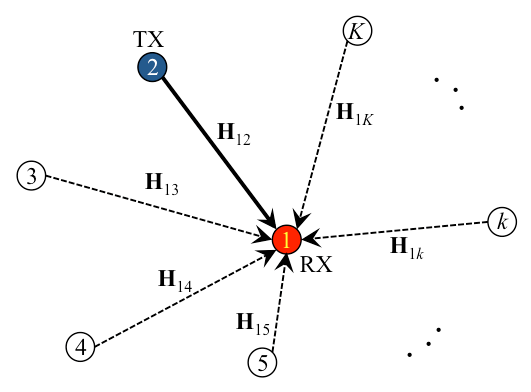
\includegraphics[width=0.5\textwidth]{../figures/InterferenceAlignment_1.png}
\caption{TBD}
\label{fig:IA_SingleRx}
\end{center}
\end{figure}

\subsubsection{Local Interference Alignment}

With the cluster head pair given, the next step in SOIA is to select other transceiver pairs from the neighborhood. These other pairs should be able to transmit at the same time with the head pair. Using IA, the interference among all pairs are under control such that the receiver of each pair can successful decode its message with high probability. 

A global optimum IA solution requires the channel knowledge from each transmitter of a cluster to all receivers in the same cluster. Instead of spending overhead resources to collect all channel information, a receiver can compute a local IA solution based on its estimated channels without considering the channels seen by other receivers. As an example, in Fig.~\ref{fig:IA_SingleRx}, the pair of node 1 and node 2 is the head pair, in which node 2 is the transmitter and node 1 is the receiver. It is reasonable to assume that each radio node in TMACN keeps track of its neighbors and the channels from these neighbors to itself. The estimates of these channels can be acquired and kept up-to-date locally. In Fig.~\ref{fig:IA_SingleRx},  radio node 1 has $K-1$ neighboring nodes. Let ${\bf{H}}_{1k}$ denote the channel between node $k$ and node 1. Node 1 can keep track of ${\bf{H}}_{1k}$ by performing channel estimations based not only on periodic beacon signals sent by node $k$, but also on any signal sent by node $k$ regardless of whether node 1 is the intended recipient. 

The algorithm for local IA is given in the following using node 1 in Fig.~\ref{fig:IA_SingleRx}. Considering the heterogeneous radio configuration in TMACN, for simplicity, we assume in the following that each radio has only 2 antennas.  
 
To align the transmissions of all neighbors, node 1 shall compute the transmission precoder vectors ${\boldsymbol{v}}_k$ for node $k=2, 3, \cdots, K$ such that
\begin{equation}\label{bfCapacity}
C_{bf}=\displaystyle\max_{{\boldsymbol{v}}_2}\log\left(1+\frac{\boldsymbol{v}_2^{*}\mathbf{H}_{12}^{*}\mathbf{H}_{12}\boldsymbol{v}_2}{\sigma^2}\right)
\end{equation}
and
\begin{equation}\label{nullbfvec}
\boldsymbol{v}_k^{*}\mathbf{H}_{1k}^{*}\mathbf{H}_{12}\boldsymbol{v}_2=\mathbf{0}, {\rm{for}}~k=3,4,\cdots~K.
\end{equation}
In Eq. (\ref{bfCapacity}), node 1 calculates the transmitter precoder vector for node 2, which maximizes the capacity between node 2 and node 1. The optimum $\boldsymbol{v}_2$ maximizing $C_{bf}$ is the one that maximizes the quadratic form $|\boldsymbol{v}_2^*\boldsymbol{\Phi}\boldsymbol{v}_2|$, where $\boldsymbol{\Phi}=\mathbf{H}_{12}^{*}\mathbf{H}_{12}$. So $\boldsymbol{v}_2$ is the eigenvector corresponding to the largest eigenvalue of $\boldsymbol{\Phi}$. Node 1 sends $\boldsymbol{v}_2$ to node 2 so the latter will use it as the transmitter beamforming vector. The desired signal space of node 2 is thus given by $\mathbf{H}_{12}\boldsymbol{v}_2$. 

In the next step, node 1 computes the beamforming vectors for all other potential interference sources in its neighborhood, i.e., node 3, 4, $\cdots~K$. More specifically, node 1 aligns all potential interference in the subspace that is orthogonal to its desired signal space. Let $\boldsymbol{v}_k$ be the transmitter beamforming vector for node k. Node 1 computes $\boldsymbol{v}_k$ such that Eq.~(\ref{nullbfvec}) holds true for nodes 3, 4, $\cdots~K$. Node 1 will broadcast vectors $\boldsymbol{v}_3$, $\boldsymbol{v}_4$, $\cdots$ $\boldsymbol{v}_K$ along with $\boldsymbol{v}_2$. Therefore, every node in the neighborhood of node 1 not only knows its own beamforming vector, but also the beamforming vector of all other nodes.

Without IA coordination, nodes 3, 4, $\cdots~K$ cannot transmit during the time slots assigned to node 2, which will use these slots to send information to node 1. By computing and broadcasting beamforming vectors $\boldsymbol{v}_3$, $\boldsymbol{v}_4$, $\cdots$ $\boldsymbol{v}_K$, node 1 provides an opportunity for some of these nodes to join the transient IA cluster headed by node 1 and 2 without impacting the transmission from node 2 to node 1. 

\subsubsection{Cluster Member Selection}
 
 
 

\subsection{Performance Analysis}


\section{PHASE I WORK PLAN}

\section{RELATED WORK}

\section{RELATIONSHIP WITH FUTURE RESEARCH OR RESEARCH AND DEVELOPMENT}

\section{COMMERCIALIZATION STRATEGY}

\section{KEY PERSONNEL}

\section{FACILITIES/EQUIPMENT}

\section{CONSULTANTS}

\section{PRIOR, CURRENT OR PENDING SUPPORT}

\bibliographystyle{IEEEtran}
\bibliography{../BibTex/ZCaoBibCollection.bib}


\end{document} 
